\documentclass[conference]{IEEEtran}
\IEEEoverridecommandlockouts
% The preceding line is only needed to identify funding in the first footnote. If that is unneeded, please comment it out.
\usepackage{cite}
\usepackage{amsmath,amssymb,amsfonts}
\usepackage{algorithmic}
\usepackage{graphicx}
\usepackage{textcomp}
\usepackage{xcolor}
\def\BibTeX{{\rm B\kern-.05em{\sc i\kern-.025em b}\kern-.08em
    T\kern-.1667em\lower.7ex\hbox{E}\kern-.125emX}}
\usepackage{booktabs}
\usepackage{fancyhdr}
\pagestyle{fancy}
\fancyhf{} 
\rfoot{\thepage}
\renewcommand{\headrulewidth}{0pt}

\begin{document}

\title{Capstone Report: Autodrone with Perception and Obstacle Avoidance}

\author{
    \IEEEauthorblockN{Jiaer Xia, Xiangxin Wan, Michael Chiu, Yanlin Jin}
    \IEEEauthorblockA{
        \textit{Department of Electrical and Computer Engineering}\\
        \textit{Rice University, Houston, TX 77005, USA}\\
        \{jx37, xw83, mc202, yj56\}@rice.edu
    }
}

\maketitle

\begin{abstract}
We aim to use AutoDrone to assist humans in performing repetitive tasks. Current state-of-the-art methods rely on various sensors (video, LiDAR, thermal) and local data processing to generate commands, often requiring significant onboard computational resources. In contrast, our approach integrates a webcam, Raspberry Pi, and 5G modem to enable lightweight perception and obstacle avoidance. By transmitting video frames over a 5G network to an external server, our system infers depth in real-time, reducing onboard computation. We demonstrate stable drone flight for over five seconds, with successful image transmission and command retrieval based on depth perception. Future work will focus on improving depth estimation accuracy, automating flight controls, and integrating advanced perception modules for enhanced performance.
\end{abstract}


\section{Introduction}
Drones have become indispensable tools across various industries, offering a unique ability to operate in environments that may be hazardous or inaccessible to humans. Their adaptability and customization allow them to serve a wide range of purposes, from delivering goods to conducting environmental surveys. One of the most critical applications of drones is in emergency response, where their deployment can significantly enhance safety and efficiency.

First responders often face life-threatening situations, such as building fires or natural disasters, where locating and rescuing victims is a priority. The integration of drones into these operations not only increases the chances of survival for those in need by delivering aid or locating them quickly but also safeguards first responders by minimizing their exposure to danger. To fulfill these roles, a drone must be capable of autonomous flight, real-time object detection using advanced sensors, mapping or imaging of the environment, and wireless communication to relay critical data back to the rescue team.

Our project focuses on developing a robust autonomous drone system designed to meet these demands. We aim to equip the drone with the ability to navigate complex environments independently, detect objects and individuals through computer vision, create detailed 3D maps, and transmit data via high-speed 5G connectivity. These features must coexist within the drone's physical and computational constraints to ensure reliable performance during flight.


\begin{figure}[h]
    \centering
    {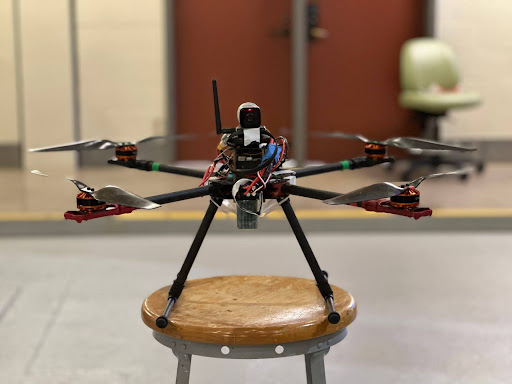
\includegraphics[scale=0.35]{figures/Drone.jpg}}
    \caption{All Equipped Drone}
    \label{Stepper Motor}
\end{figure}


\section{Methods}

\subsection{Hardware}

\subsubsection{Drone}

In the AutoDrone project, the system consists of two main components: the Raspberry Pi and the Flight Control Unit (FCU). The FCU integrates sensors such as gyroscopes, accelerometers, and temperature sensors, manages GPS input, and distributes power to the motors, serving as the drone's core navigation and stability controller.

The Raspberry Pi acts as the main computational controller, processing data from the onboard camera and LiDAR systems. Using optimized deep learning algorithms, it performs tasks like person re-identification and object tracking by interpreting depth information to guide the FCU for precise maneuvering in dynamic environments.

To maximize the Raspberry Pi’s performance within hardware limits, lightweight neural networks and inference tools like TensorFlow Lite and OpenCV's deep learning modules are employed. Extensive testing is being conducted under various conditions, such as lighting changes, GPS signal fluctuations, and environmental noise, to evaluate performance, latency, accuracy, and power consumption.

\subsubsection{Hardware Debugging and Stabilization}
Ensuring stable and reliable flight for the AutoDrone system required careful attention to debugging and stabilizing the drone's hardware. A key part of this process involved balancing the drone's center of gravity and ensuring proper alignment to maintain stability during flight.

A bubble level was used to verify that all four propellers were parallel to the ground, minimizing aerodynamic imbalances that could compromise stability. Additionally, the drone’s center of gravity was manually measured and adjusted by repositioning components such as the battery, flight controller, and sensors. This ensured even weight distribution and maintained the center of gravity at the physical center of the drone, preventing unintentional tilting or drift.


\subsubsection{5G}
 For our project, The host is a Raspberry Pi 3 Model B+ that is running Raspberry Pi OS released 2024-07-04. For 5G, we use a Sixfab 5G Raspberry Pi Modem. The physical form factor is designed to easily connect to a Raspberry Pi but the module is compatible with Linux and Windows systems. The modem has a Quectel RM502Q-AE chip capable of 5G SA communication. For testing our wireless connectivity, we used an implementation of a OpenAirInterface (OAI) 5G SA network using a Foxconn RU. We used both OpenCell and Sysmocom SIM cards that we programmed ourselves for use on our network. 

\subsection{Wireless Data Transfer}
To establish connectivity, we intially used ICMP traffic to validate device connection. To ensure stability, we tested bandwidth at varying rates and periods of times. After establishing one device, we began testing multiple devices with simultaneous connections. We first validated that the drone (Raspberry Pi) could transmit data between itself and the network containers over 5G. Once successful, we injected next hop routes on the devkit servers to complete the route from the Raspberry pi to devkit02 over 5G. As seen in Fig.~\ref{NetDiag}, traffic must traverse Argosnet for traffic to leave devkit01 which hosts the 5G containers. 



To handle the data transfer between the drone's Raspberry Pi and the server, we used Python scripts on each end to create a UDP socket and iterate through a loop. Prior to starting the respective loops, the client would initialize the camera and the server would generate the model for the depth estimation. The client captured an image using a webcam attached via USB-A and would resize the image a create a JPG about 45 KB. The client loop would then read the image as a bytestring and send via the UDP socket until complete, which the loop would then listen for the response from the server. Once the response was received, it would start the loop over and take another image until the number of iterations was complete. On the server end, the loop waited to receive the file and wrote the bytestring to a JPG file. The loop then called the depth estimation model on the received JPG and generated the depth map. Once generated, the loop sent the mean depth value to the client over the UDP socket and waited to receive the next image. 

\begin{figure}[h]
    \centering
    {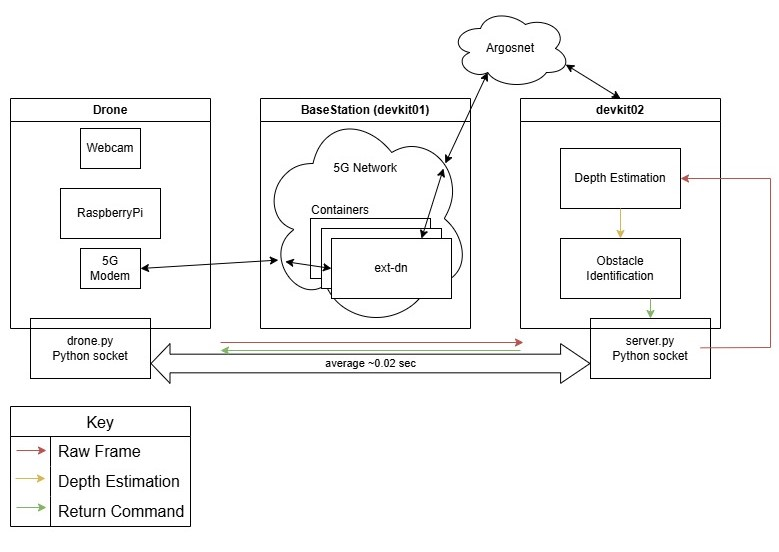
\includegraphics[scale=0.5]{ELEC594 Autodrone project final report/figures/ObsDet_Diagram.jpg}}
    \caption{Network Diagram}
    \label{NetDiag}
\end{figure}

\subsection{3D Reconstruction and Trajectory Localization}
We use the video data collected by the drone to reconstruct 3D point clouds of the scene and simultaneously obtain the drone's motion trajectory. The reconstruction process starts with key point extraction, where we use the SIFT \cite{SIFT} algorithm. Then we match the feature points in overlapping views by measuring the similarity between key point descriptors. After matching, a screening process is applied to filter outliers using RANSAC~\cite{Ransac}. Finally, the 3D point cloud and camera poses are jointly estimated through a process that alternates between structure estimation and motion estimation. Bundle adjustment~\cite{ba} is applied globally, optimizing both the camera parameters and 3D points to minimize reprojection error across all images. Through this structure from motion process, we now have the reconstructed point clouds and an estimated camera trajectory.

We also tried end-to-end deep visual odometry to obtain camera ego-motion trajectories~\cite{scsfm}. The deep visual odometry model is usually trained in a self-supervised manner by simultaneously predicting the depth and relative camera transformation and then use the reprojection error to constrain the training. However, in our case, the video data captured by the drone is limited by low frame rate and resolution, making it unsuitable for training purposes. Consequently, we trained the model with the Kitti dataset~\cite{kitti} and tested on our data. The model performs poorly due to the large domain gap between the training and testing dataset. A possible solution is to train the model on publicly available drone-captured datasets. However, this may be time-consuming due to the need for data format adjustments, and there could still be a significant domain gap between other drones' data and ours. Therefore, we still chose to use the Structure-from-Motion~\cite{colmap} approach to obtain trajectories, as it is a relatively robust offline method when the camera undergoes enough translation and rotation.

\subsection{Obstacle Avoidance}
To prevent the drone from potentially colliding with obstacles, we developed an obstacle avoidance perception algorithm based on depth information. We employed DepthAnythingV2 for depth prediction. DepthAnythingV2~\cite{depthanything} is an open-source, large-scale model trained on both labeled and extensive unlabeled datasets. We selected the smallest model to estimate the depth of frames captured by the drone for real-time performance. Our perception decision algorithm calculates the average depth of the central region of the predicted depth map. This region corresponds to the central area where both the width and height are each \( \frac{1}{2} \) of the map's total dimensions. Specifically, let \( C \subset D \) represent this central area:

\[
C = D\left(\frac{w}{4} : \frac{3w}{4}, \frac{h}{4} : \frac{3h}{4}\right),
\]

where \( D \in \mathbb{R}^{w \times h} \) is the depth map. The average depth is computed as: 

\[
\text{Average Depth} = \frac{1}{|C|} \sum_{(x, y) \in C} D(x, y).
\]

If the average depth value exceeds \( 128 \), a collision risk alert is activated. Otherwise, the area is considered safe. This is a relatively simple approach, especially given that the model predicts only relative depth. However, it has been successful in most tested scenarios.


\subsection{Panotic Segmentation with GroundedSAM}
GroundedSAM is an innovative segmentation method that integrates the zero-shot detection capabilities of Grounding DINO with the flexible segmentation features of the Segment Anything Model (SAM), enabling precise object segmentation guided by text-based prompts.
\begin{itemize}
    \item \textbf{Grounding DINO\cite{Grounding dino}:} Grounding DINO serves as an open-set object detector, capable of interpreting free-form text descriptions to locate objects within an image. Built on Vision Transformers (ViTs), it leverages pretraining on large-scale unlabeled datasets to achieve robust visual representation learning. This empowers Grounding DINO to generalize effectively to unseen object categories, producing accurate bounding boxes and labels.
    \item \textbf{Segment Anything Model (SAM)\cite{SAM}:} SAM is a foundational segmentation model capable of segmenting any distinguishable entity in an image based on point, bounding box, or text prompts. It employs a Transformer-based image encoder to process visual inputs into feature embeddings, which are then combined with prompt embeddings to generate precise segmentation masks.
    \item \textbf{Integration in GroundedSAM\cite{GroundedSAM}:}  By combining Grounding DINO and SAM, GroundedSAM first utilizes Grounding DINO's detection capabilities to identify target objects within an image using text-based prompts. The resulting bounding boxes serve as inputs to SAM, which then produces accurate segmentation masks for the detected objects. This synergy between detection and segmentation ensures robust performance in diverse and complex visual scenarios.
\end{itemize}

\begin{figure}[h]
    \centering
    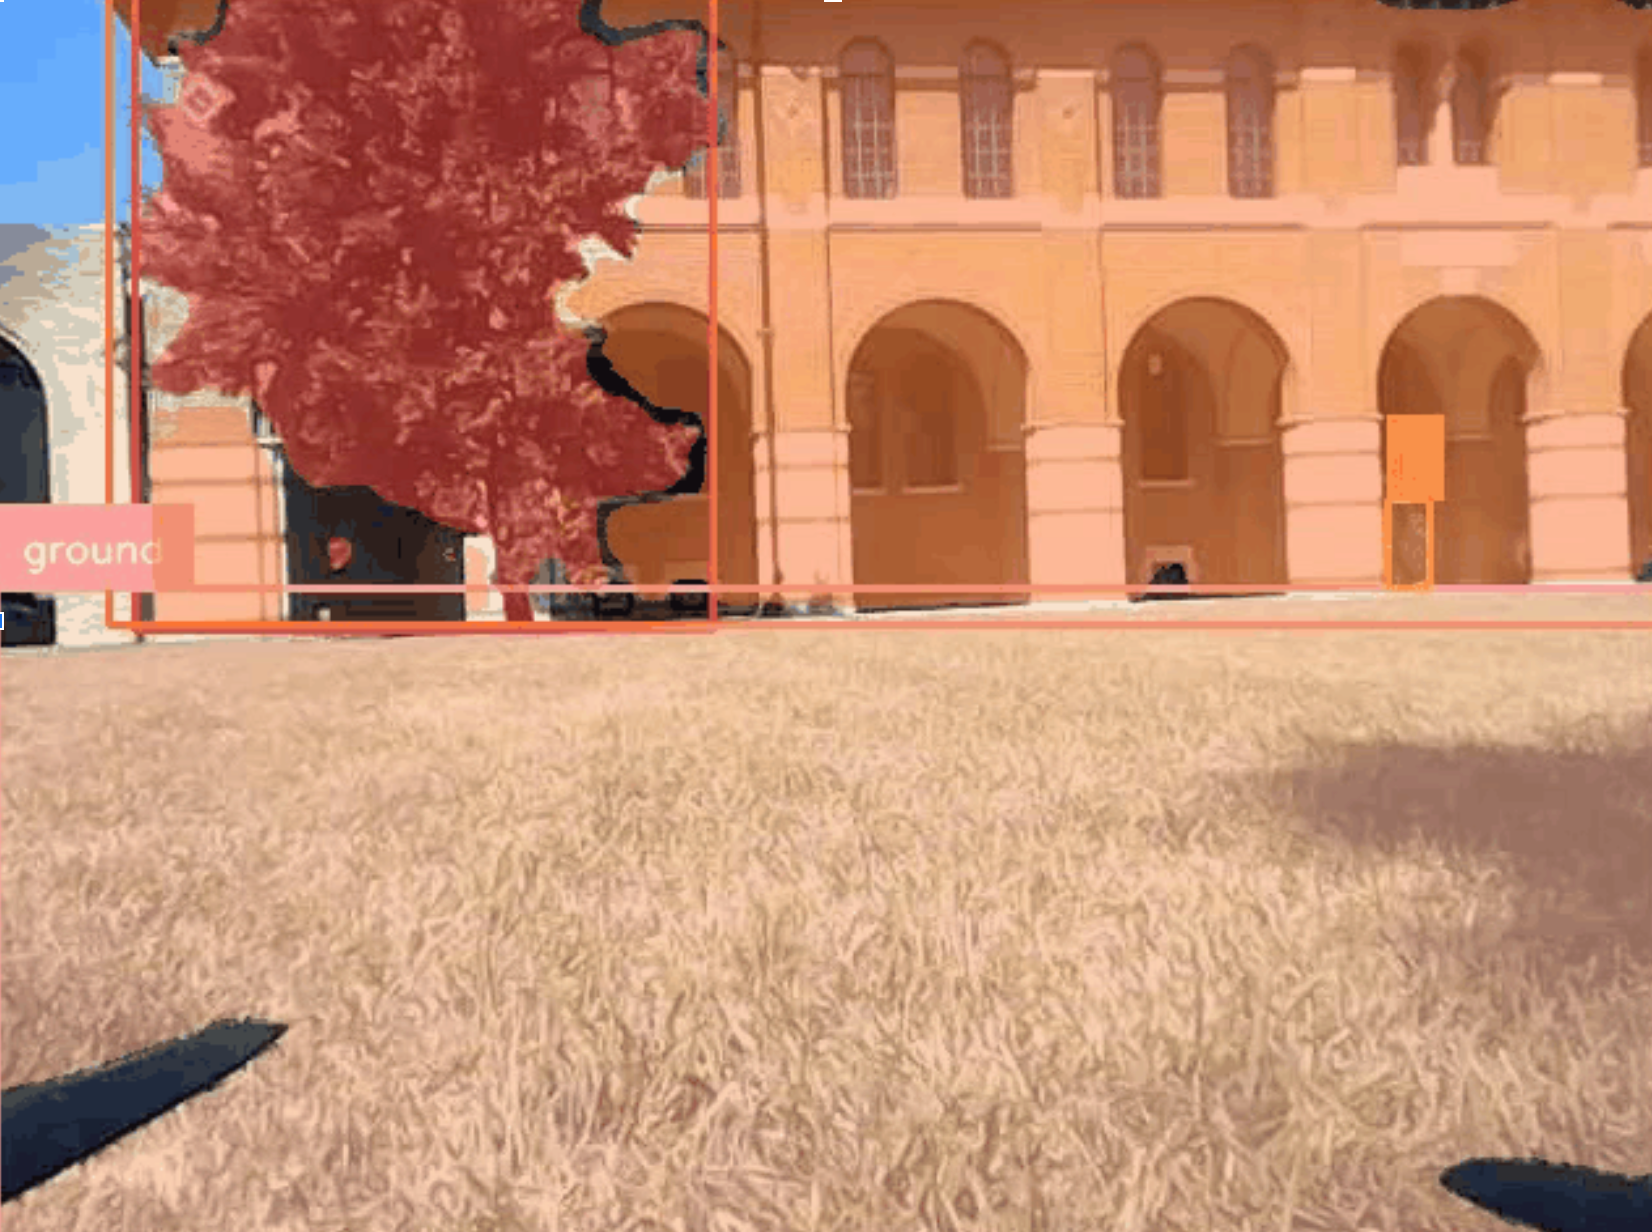
\includegraphics[width=0.8\columnwidth]{ELEC594 Autodrone project final report/figures/segmentation.jpg}
    \caption{Panotic Segmentation with GroundedSAM}
    \label{fig:segmentation}
\end{figure}

\section{Results}
\subsection{Wireless Data Transfer}
To justify the wireless transmission of data, we need to validate that the increased speed of depth estimation achieved a greater performance advantage than the round trip time to complete the transfer. In Table~\ref{tab:depth times}, we show the time it took to run the depth inference once on three different machines: a Raspberry Pi (Device Edge), a laptop (network edge), and a server (enterprise edge). The total time also includes the time to generate the model. We optimized the way the server call the depth inference so that it generates the model prior to starting the loop and reuses the model with each iteration.

\begin{table}[h]
\centering
\caption{Depth Estimation Times}
\label{tab:depth times}
\begin{tabular}{lcc}
\toprule
 & \textbf{Depth Inference (seconds)} & \textbf{Total Time (seconds)} \\ \midrule
\textbf{Raspberry Pi} & 95.8370 & 116.8748\\
\textbf{Laptop} & 1.1008 & 2.0020  \\
\textbf{Server (devkit02)} & 0.0411 & 0.8755  \\ 
\bottomrule
\end{tabular}
\end{table}

To test, we iterated through the script loop 5 times with no injected wait time between iterations. Table~\ref{tab:data times} shows iteration times as well as the average time for the 5 iterations. Based on our testing, we are able to process images on the server by sending over 5G approximately 5 times faster than the image could be processed on a laptop. By transmitting over 5G and processing on the edge server, we are able to send 5 commands to the drone every second to control its flight. 

\begin{table}[h]
\centering
\caption{Data Transfer Times}
\label{tab:data times}
\begin{tabular}{lcccccc}
\toprule
 & \textbf{Iter 1} & \textbf{Iter 2} & \textbf{Iter 3} & \textbf{Iter 4} & \textbf{Iter 5} & \textbf{Avg Time} \\ \midrule
\textbf{Test 1 (sec)} & 0.5106 & 0.1685 & 0.0913 & 0.0904 & 0.1697 & 0.2061 \\
\textbf{Test 2 (sec)} & 0.4532 & 0.1766 & 0.0952 & 0.0960 & 0.0964 & 0.1835 \\
\textbf{Test 3 (sec)} & 0.4486 & 0.1724 & 0.0908 & 0.1728 & 0.0900 & 0.1949 \\ 
\bottomrule
\end{tabular}
\end{table}




\subsection{3D Reconstruction and Trajectory Localization}
We extracted 75 frames from a relatively successful flight for the experiment, obtaining a reasonable drone trajectory and a sparse reconstruction result. The red line in the Fig.~\ref{fig:reconstruction} illustrates the drone's trajectory as it ascends and then descends along a curved path. The surrounding point cloud also reconstructs the original environment and the distant buildings.
\begin{figure}[h]
    \centering
    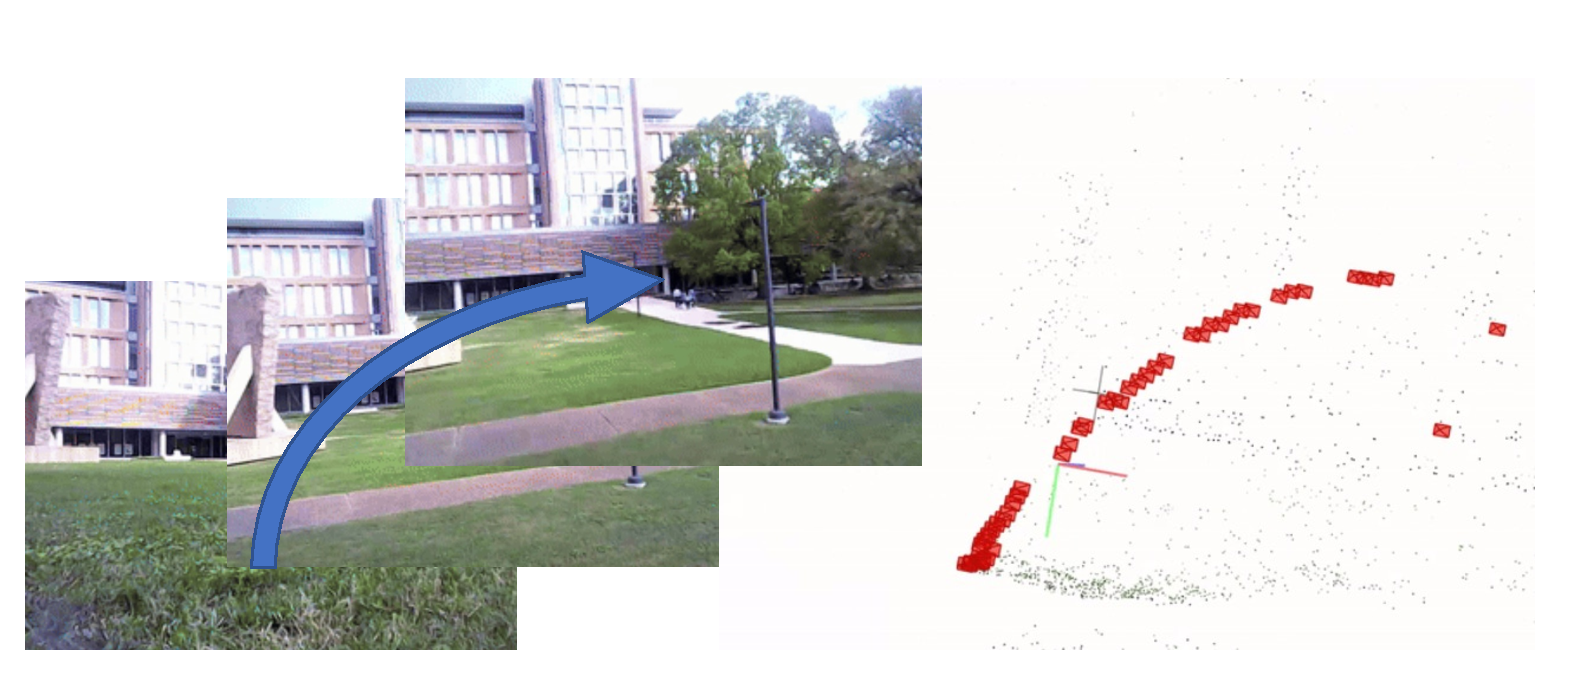
\includegraphics[width=\columnwidth]{figures/reconstruction.pdf}
    \caption{Trajectory and Sparse Reconstruction}
    \label{fig:reconstruction}
\end{figure}


\subsection{Obstacle Avoidance}
We set up a simple test scenario to verify the effectiveness of the algorithm. Four photos were taken at distances of 150 cm, 120 cm, 90 cm, and 60 cm, simulating the drone approaching an obstacle as shown in Fig.~\ref{fig:perception}. The average depth within the red central rectangular region was then calculated for each photo. We present the average pixel values within the red bounding box in Table~\ref{tab:perception}, along with a single pixel value on the central object. We observed that relying on a single pixel is inaccurate due to the relative nature of the used depth model. However, calculating the average pixel value within the box provides a better indication of nearby objects. This approach is still very basic. Our proposed future improvements include using a model fine-tuned on absolute depth scale and integrating object detection and segmentation for more precise perception.

\begin{figure}[h]
    \centering
    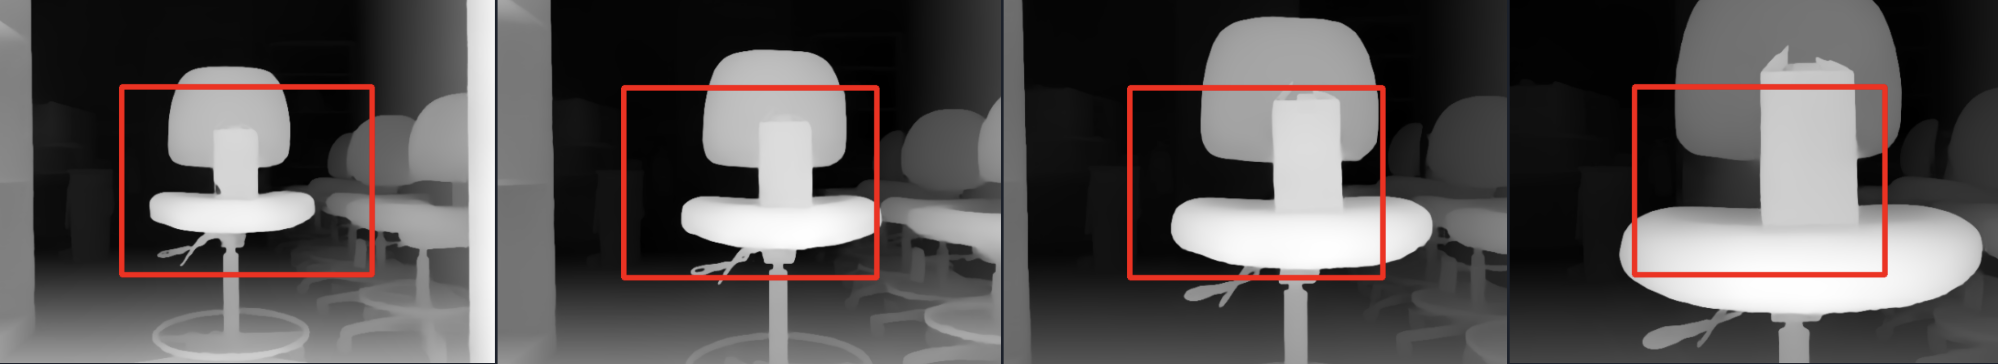
\includegraphics[width=\columnwidth]{figures/perception.png}
    \caption{Depth estimation results as the drone approaches the objects}
    \label{fig:perception}
\end{figure}

\begin{table}[h]
\centering
\caption{Depth Values and returned Commands}
\label{tab:perception}
\begin{tabular}{lcccc}
\toprule
 & \textbf{150 cm} & \textbf{120 cm} & \textbf{90 cm} & \textbf{60 cm} \\ \midrule
\textbf{Central Pixel Value} & 213.0 & 221.0 & 219.0 & 203.0 \\
\textbf{Average Depth Value} & 93.63 & 105.95 & 131.22 & 148.73 \\
\textbf{Command}             & Safe  & Safe   & Stop   & Stop   \\ 
\bottomrule
\end{tabular}
\end{table}


\section{Discussion}
\subsection{Limitations}

The AutoDrone project has shown promising progress toward creating an autonomous drone system capable of navigating hazardous environments. However, several limitations affect its performance, scalability, and real-world deployment:

\subsubsection{Communication Reliability and Computational Constraints}
The system relies on 5G communication to transmit sensor data to cloud servers for computationally intensive tasks like object detection and 3D reconstruction. This approach compensates for the Raspberry Pi's limited processing power but introduces dependency on stable 5G coverage. Weak signals or network instability could delay communication and real-time processing.

\subsubsection{Environmental Variability}
The system's performance can be impacted by environmental factors such as variable lighting, smoke, fog, strong winds, and rain. These conditions affect camera and LiDAR accuracy, impair object detection, and reduce flight stability, limiting overall system reliability.

\subsubsection{Battery and Flight Time Limitations}
While the drone's battery performs well during initial takeoff, performance declines over extended use due to power depletion. Prolonged flight causes reduced lift, limiting the drone's ability to sustain operations for extended emergency response scenarios.

\subsubsection{Sensor and Hardware Integration Challenges}
Integrating multiple sensors, such as cameras, LiDAR, and GPS, requires precise calibration and synchronization. Misalignment, interference, or processing delays can still occur, impairing navigation and decision-making.

\subsubsection{Testing Environments vs. Real-World Scenarios}
Although testing has been performed under various controlled conditions, real-world deployment introduces additional unpredictability, including changing weather, unexpected obstacles, and varying terrains, which could affect system reliability.

\subsection{Future Works}
\paragraph{Tryp: A Potential Training Tool}
This semester, the team encountered numerous challenges during flight tests, including frequent crashes that necessitated repeated repairs to the drone. These difficulties highlighted the need for an alternative training method to enhance pilot skills while minimizing damage to the drone. Moving forward, we propose integrating FPV (First-Person View) flight simulators, such as \textit{Tryp} and \textit{Uncrashed}, into our training and development workflows. These simulators are widely regarded as essential tools for FPV pilots, offering realistic physics modeling and immersive environments to refine skills and optimize drone performance.


\textit{Tryp} is a professional FPV simulator designed to facilitate pilot training and drone development. With its advanced features, it serves as a robust platform for both beginners and experienced developers. Below, we outline the key features that make \textit{Tryp} particularly valuable:

\begin{itemize}
    \item \textbf{Highly Realistic Physics Simulation:} \textit{Tryp} accurately simulates aerodynamics, gravity, thrust control, and other flight dynamics, providing a true-to-life experience of drone behavior.
    \item \textbf{Diverse Flight Scenarios:} Users can practice in a range of virtual environments, such as urban landscapes, forests, and racing tracks, fostering adaptability in various conditions. These maps can simulate diverse terrains and operational challenges, providing invaluable experience for both novice and advanced pilots.
    \item \textbf{Customizable Drone Parameters:} \textit{Tryp} allows for the customization of parameters such as thrust, weight distribution, propeller sizes, and motor configurations. This flexibility enables us to simulate the exact specifications of our project’s drone, allowing for targeted performance evaluations and adjustments before real-world deployment.
    \item \textbf{Support for Multiple Control Devices:} \textit{Tryp} supports popular remote controllers and simulator hardware, ensuring a hands-on experience that closely mirrors real-world operations.
    \item \textbf{Community and Competition Modes:} The platform includes online collaboration features and competitive racing modes, fostering skill development through engagement with a global FPV community.
\end{itemize}

Incorporating FPV simulators into the project’s training process could significantly reduce the risk of drone damage during practice sessions while providing a more efficient and cost-effective approach to pilot training. The ability to freely adjust drone parameters in \textit{Tryp} allows us to simulate our specific drone model, ensuring a high degree of relevance and precision in our testing. Additionally, the availability of diverse maps provides a safe and controlled environment for testing navigation and maneuvering in various scenarios. As the project evolves, leveraging these simulators is expected to play a crucial role in enhancing the technical and operational expertise of the team, ultimately contributing to the success of future drone applications.

\begin{figure}[h]
    \centering
    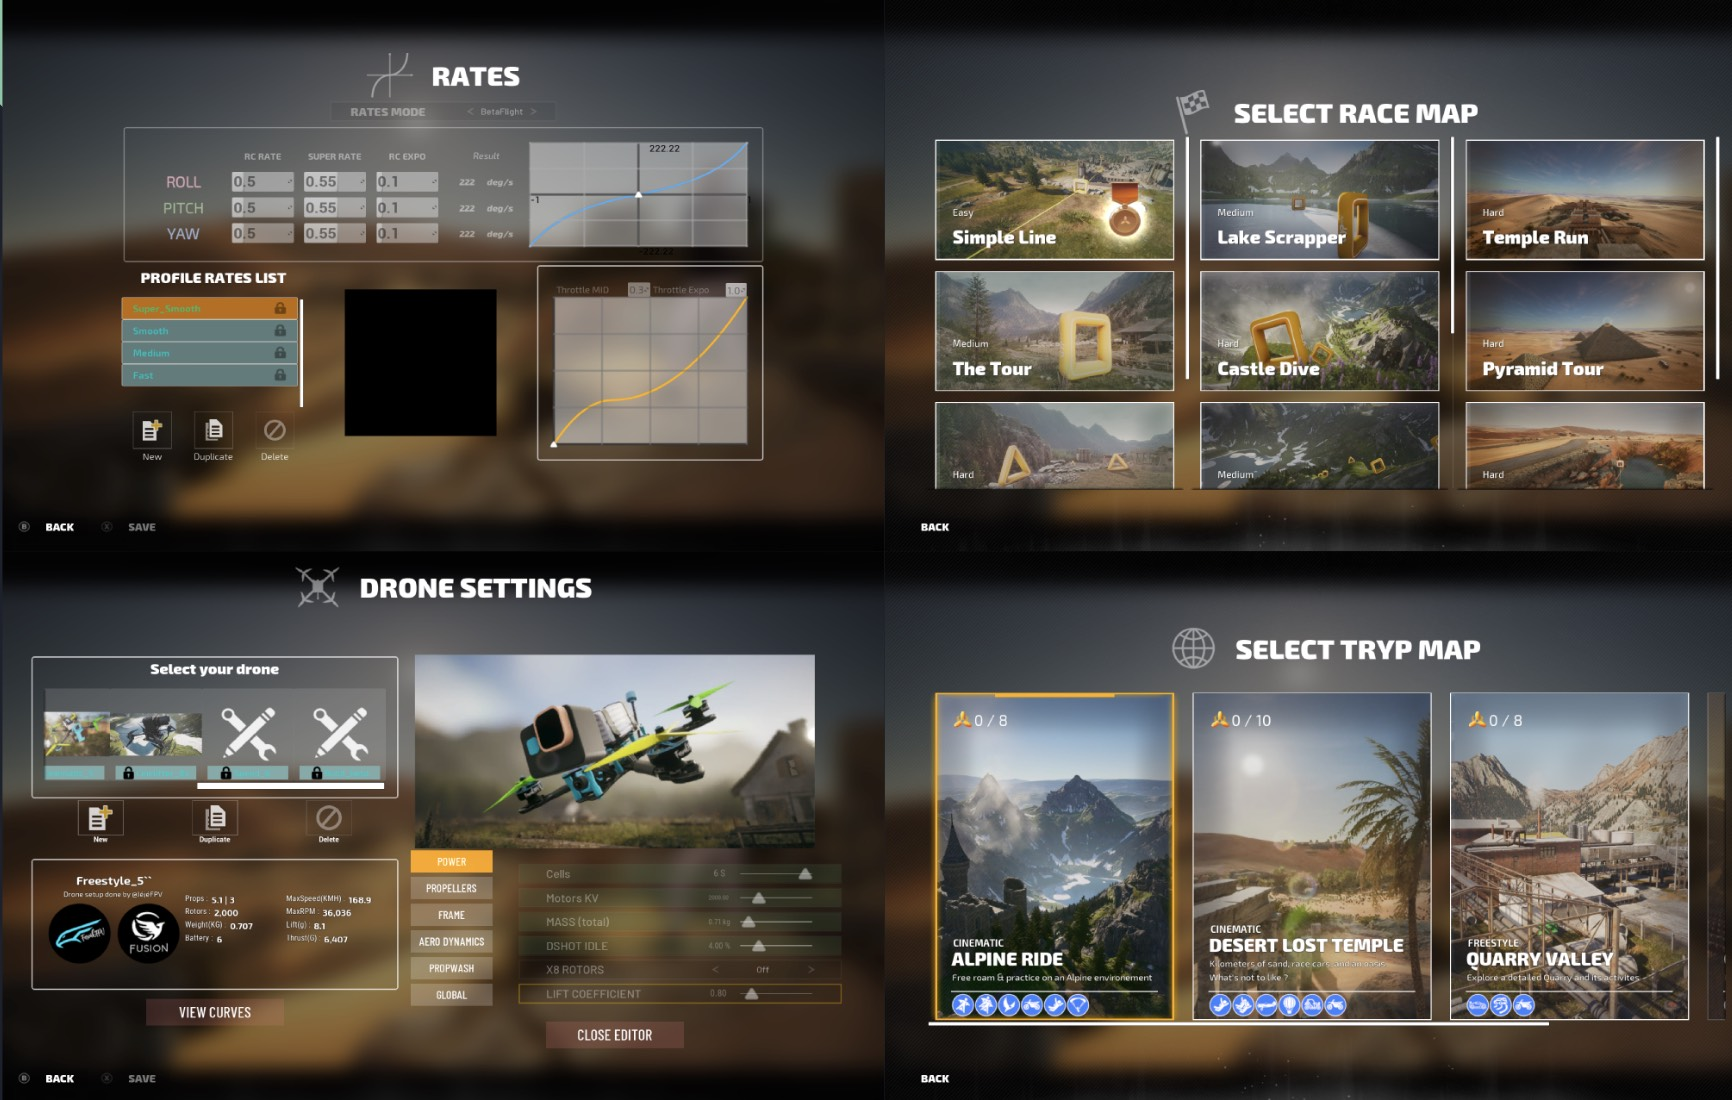
\includegraphics[width=0.8\columnwidth]{ELEC594 Autodrone project final report/figures/Tryp-interface.jpg}
    \caption{Tryp Interface}
    \label{fig:tryp}
\end{figure}

\paragraph{Image Transmission Optimization}
We conducted 5 iteration rounds across multiple network setups, achieving consistent success. However, prolonged use increased round trip time variability. Future testing should explore burst transmissions and artificial wait periods. To maximize efficiency, drone responsiveness should be measured to determine the minimum viable round trip time, ensuring commands are sent at a rate the drone can handle. This approach could improve speed and reduce latency.

Error handling in image transmission should also be enhanced. If too many packets are dropped, making the image unusable for depth inference, the system should resynchronize instead of stalling, allowing the server and drone to recover and proceed with new data.

\section{Conclusion}
In this project, we successfully developed an autonomous drone system tailored to emergency response applications. By integrating advanced technologies such as optimized object detection algorithms, 3D reconstruction using LiDAR, and high-speed 5G communication, the system demonstrates significant capabilities in navigation, perception, and environmental modeling. Despite challenges such as computational limitations, environmental variability, and flight constraints, the project highlights the potential for drones to enhance safety and operational efficiency in hazardous environments.

Our results, including reliable obstacle avoidance, real-time depth estimation, and effective trajectory localization, underline the practicality of our approach. Future efforts will address current limitations, such as improving robustness against environmental factors and extending battery life, while exploring enhanced training tools and fine-tuned models for more complex scenarios. This research lays a foundation for continued innovation in autonomous drone systems, bridging gaps between theoretical advancements and real-world applications.

\section*{Acknowledgements}
This research was made possible by the generous financial support from the Rice University Electrical and Computer Department, to whom we extend our heartfelt gratitude. We are also deeply grateful to Prof. Jose Moreto and Prof. Joseph Young for their guidance.

% We owe a profound debt of gratitude to Dr. Joseph Young, our mentor for the Autodrone project, for his invaluable guidance and expert advice throughout the duration of this project. On behalf of the entire team, we also extend our heartfelt thanks to Dr. Rahman Doost for his invaluable support and expertise in 5G communications, which greatly enhanced our project. Our sincere thanks also go to the former members of the Autodrone project, whose pioneering work laid the groundwork for our research. Their contributions have been instrumental in achieving the outcomes presented in this study.



% Please number citations consecutively within brackets \cite{b1}. The 
% sentence punctuation follows the bracket \cite{b2}. Refer simply to the reference 
% number, as in \cite{b3}---do not use ``Ref. \cite{b3}'' or ``reference \cite{b3}'' except at 
% the beginning of a sentence: ``Reference \cite{b3} was the first $\ldots$''

% Number footnotes separately in superscripts. Place the actual footnote at 
% the bottom of the column in which it was cited. Do not put footnotes in the 
% abstract or reference list. Use letters for table footnotes.

% Unless there are six authors or more give all authors' names; do not use 
% ``et al.''. Papers that have not been published, even if they have been 
% submitted for publication, should be cited as ``unpublished'' \cite{b4}. Papers 
% that have been accepted for publication should be cited as ``in press'' \cite{b5}. 
% Capitalize only the first word in a paper title, except for proper nouns and 
% element symbols.

% For papers published in translation journals, please give the English 
% citation first, followed by the original foreign-language citation \cite{b6}.

\begin{thebibliography}{00}
\bibitem{SIFT} Lowe, David G. "Object recognition from local scale-invariant features." Proceedings of the seventh IEEE international conference on computer vision. Vol. 2. Ieee, 1999.
\bibitem{Ransac} Fischler, Martin A., and Robert C. Bolles. "Random sample consensus: a paradigm for model fitting with applications to image analysis and automated cartography." Communications of the ACM 24.6 (1981): 381-395.
\bibitem{ba} Triggs, Bill, et al. "Bundle adjustment—a modern synthesis." Vision Algorithms: Theory and Practice: International Workshop on Vision Algorithms Corfu, Greece, September 21–22, 1999 Proceedings. Springer Berlin Heidelberg, 2000.
\bibitem{kitti} Geiger, Andreas, et al. "Vision meets robotics: The kitti dataset." The International Journal of Robotics Research 32.11 (2013): 1231-1237.
\bibitem{colmap} Schonberger, Johannes L., and Jan-Michael Frahm. "Structure-from-motion revisited." Proceedings of the IEEE conference on computer vision and pattern recognition. 2016.
\bibitem{depthanything} Yang, Lihe, et al. "Depth Anything V2." arXiv preprint arXiv:2406.09414 (2024).
\bibitem{scsfm} Bian, Jiawang, et al. "Unsupervised scale-consistent depth and ego-motion learning from monocular video." Advances in neural information processing systems 32 (2019).
\bibitem{GroundedSAM}Ren, Tianhe, et al. "Grounded sam: Assembling open-world models for diverse visual tasks." arXiv preprint arXiv:2401.14159 (2024).
\bibitem{Grounding dino}Liu, Shilong, et al. "Grounding dino: Marrying dino with grounded pre-training for open-set object detection." European Conference on Computer Vision. Springer, Cham, 2025.
\bibitem{SAM}Kirillov, Alexander, et al. "Segment anything." Proceedings of the IEEE/CVF International Conference on Computer Vision. 2023.
\end{thebibliography}
\vspace{12pt}


\end{document}
